\documentclass[aspectratio=169,11pt]{beamer}

% =========================================================
% Theme
% =========================================================
\usetheme{Madrid}
\usecolortheme{seahorse}
\setbeamertemplate{navigation symbols}{}

% =========================================================
% Packages
% =========================================================
\usepackage[utf8]{inputenc}
\usepackage[T1]{fontenc}
\usepackage{lmodern}
\usepackage{amsmath,amssymb}
\usepackage{xcolor}
\usepackage{booktabs}
\usepackage{array}
\usepackage{listings}
\usepackage{tikz}
\usetikzlibrary{arrows.meta,positioning,fit,calc,shapes.geometric}
\usepackage{hyperref}
\hypersetup{pdfpagemode=UseNone}

% =========================================================
% Colors
% =========================================================
\definecolor{deepblue}{RGB}{0,51,102}
\definecolor{softblue}{RGB}{220,235,247}
\definecolor{softgreen}{RGB}{223,242,228}
\definecolor{softorange}{RGB}{255,238,214}
\definecolor{softred}{RGB}{252,228,228}
\definecolor{codebg}{RGB}{248,248,248}
\definecolor{mygray}{RGB}{90,90,90}
\definecolor{mypurple}{RGB}{102,0,153}

% =========================================================
% Listings
% =========================================================
\lstset{
	language=Java,
	basicstyle=\ttfamily\small,
	backgroundcolor=\color{codebg},
	frame=single,
	breaklines=true,
	columns=fullflexible,
	showstringspaces=false,
	keywordstyle=\color{deepblue}\bfseries,
	commentstyle=\color{green!50!black},
	stringstyle=\color{mypurple},
	numbers=left,
	numberstyle=\tiny\color{mygray},
	stepnumber=1,
	numbersep=8pt
}

% =========================================================
% Title Info
% =========================================================
\title[Week 4 -- Part 4]{Concurrency and Distributed Systems}
\subtitle{Week 4 -- Part 4: AtomicInteger, CAS, Lock-Free Programming, and Contention}
\author{Dr. Mohamad Aoude}
\institute{Faculty of Engineering}
\date{\today}

% =========================================================
% Custom Blocks
% =========================================================
\setbeamercolor{block title}{bg=deepblue!85, fg=white}
\setbeamercolor{block body}{bg=softblue, fg=black}

\setbeamercolor{alertblock title}{bg=red!75!black, fg=white}
\setbeamercolor{alertblock body}{bg=softred, fg=black}

\setbeamercolor{exampleblock title}{bg=green!50!black, fg=white}
\setbeamercolor{exampleblock body}{bg=softgreen, fg=black}

% =========================================================
% Footer
% =========================================================
\setbeamertemplate{footline}{
	\leavevmode
	\hbox{
		\begin{beamercolorbox}[wd=.78\paperwidth,ht=2.5ex,dp=1.2ex,leftskip=0.3cm]{author in head/foot}
			\usebeamerfont{author in head/foot}Concurrency and Distributed Systems --- Week 4 Part 4
		\end{beamercolorbox}
		\begin{beamercolorbox}[wd=.22\paperwidth,ht=2.5ex,dp=1.2ex,rightskip=0.3cm]{date in head/foot}
			\hfill \insertframenumber/\inserttotalframenumber
		\end{beamercolorbox}
	}
}

% =========================================================
% Document
% =========================================================
\begin{document}
	
	% =========================================================
	\begin{frame}
		\titlepage
	\end{frame}
	
	% =========================================================
	\begin{frame}{Part 4 Roadmap}
		\tableofcontents
	\end{frame}
	
	\section{Why We Need Another Tool}
	\section{AtomicInteger}
	\section{Compare-And-Swap (CAS)}
	\section{Lock-Free Programming Intuition}
	\section{Performance and Contention}
	\section{Comparison with Locks}
	\section{Lab Preparation and Week Summary}
	
	% =========================================================
	\begin{frame}{Where We Are in Week 4}
		\begin{block}{Part 1}
			We learned why threads can observe stale values.
		\end{block}
		
		\vspace{0.2cm}
		
		\begin{block}{Part 2}
			We learned that \texttt{volatile} provides:
			\begin{itemize}
				\item visibility
				\item ordering
				\item happens-before through volatile communication
			\end{itemize}
		\end{block}
		
		\vspace{0.2cm}
		
		\begin{block}{Part 3}
			We learned that visibility is not enough:
			\begin{itemize}
				\item \texttt{counter++} is not atomic
				\item lost updates happen
				\item DCL needs both locking and safe publication
			\end{itemize}
		\end{block}
		
		\vspace{0.2cm}
		
		\begin{alertblock}{Now Part 4 asks}
			How can we perform atomic shared-state updates \emph{without} relying on a traditional lock for every operation?
		\end{alertblock}
	\end{frame}
	
	% =========================================================
	\begin{frame}{Learning Objectives}
		By the end of this lecture, students should be able to:
		
		\begin{itemize}
			\item explain why \texttt{AtomicInteger} solves a different problem than \texttt{volatile}
			\item use \texttt{AtomicInteger} for correct atomic increments
			\item explain the idea of compare-and-swap (CAS)
			\item understand retry-based optimistic update logic
			\item define lock-free programming at an introductory level
			\item compare atomic variables with locks from Week 3
			\item reason about performance under contention
		\end{itemize}
	\end{frame}
	
	% =========================================================
	\begin{frame}{Why We Need Another Tool}
		After Part 3, students should already know:
		
		\begin{itemize}
			\item a plain shared counter is unsafe
			\item a volatile counter is still unsafe
			\item locks can make the counter safe
		\end{itemize}
		
		\vspace{0.35cm}
		
		\begin{exampleblock}{Natural next question}
			Can we get a correct atomic increment without surrounding every update with a traditional lock?
		\end{exampleblock}
		
		\vspace{0.3cm}
		
		\begin{block}{Answer}
			Yes, for many cases Java provides atomic classes such as:
			\[
			\texttt{AtomicInteger}
			\]
		\end{block}
	\end{frame}
	
	% =========================================================
	\begin{frame}[fragile]{The Basic AtomicInteger Example}
		\begin{lstlisting}
			import java.util.concurrent.atomic.AtomicInteger;
			
			class AtomicCounterDemo {
				static AtomicInteger counter = new AtomicInteger(0);
				
				static void increment() {
					counter.incrementAndGet();
				}
			}
		\end{lstlisting}
		
		\vspace{0.25cm}
		
		\begin{block}{Why this matters}
			This performs an atomic read-modify-write update on the shared value.
		\end{block}
		
		\vspace{0.25cm}
		
		\begin{alertblock}{Important}
			This is not just ``a visible int.''  
			It is an object that provides atomic operations.
		\end{alertblock}
	\end{frame}
	
	% =========================================================
	\begin{frame}{AtomicInteger vs volatile int}
		\centering
		\begin{tabular}{>{\bfseries}m{3.2cm} >{\centering\arraybackslash}m{2cm} >{\centering\arraybackslash}m{2cm} >{\centering\arraybackslash}m{2cm}}
			\toprule
			Mechanism & Visibility & Ordering & Atomic Increment \\
			\midrule
			\texttt{volatile int} & Yes & Yes & No \\
			\texttt{AtomicInteger} & Yes & Yes & Yes \\
			\bottomrule
		\end{tabular}
		
		\vspace{0.4cm}
		
		\begin{exampleblock}{Interpretation}
			\texttt{AtomicInteger} does not merely expose a value.  
			It exposes operations with stronger guarantees.
		\end{exampleblock}
	\end{frame}
	
	% =========================================================
	\begin{frame}[fragile]{A Complete Atomic Counter Example}
		\begin{lstlisting}
			import java.util.concurrent.atomic.AtomicInteger;
			
			public class AtomicCounterDemo {
				static AtomicInteger counter = new AtomicInteger(0);
				
				public static void main(String[] args) throws Exception {
					Thread t1 = new Thread(() -> {
						for (int i = 0; i < 100000; i++) {
							counter.incrementAndGet();
						}
					});
					
					Thread t2 = new Thread(() -> {
						for (int i = 0; i < 100000; i++) {
							counter.incrementAndGet();
						}
					});
					
					t1.start();
					t2.start();
					t1.join();
					t2.join();
					
					System.out.println(counter.get());
				}
			}
		\end{lstlisting}
	\end{frame}
	
	% =========================================================
	\begin{frame}{What Makes This Work?}
		\begin{block}{Key idea}
			\texttt{AtomicInteger} provides operations that behave atomically with respect to concurrent updates.
		\end{block}
		
		\vspace{0.3cm}
		
		So for:
		\[
		\texttt{counter.incrementAndGet()}
		\]
		
		we do \emph{not} get the unsafe pattern:
		
		\begin{itemize}
			\item read shared value
			\item compute locally
			\item race during write-back
		\end{itemize}
		
		\vspace{0.3cm}
		
		\begin{exampleblock}{Instead}
			The update is executed using a lower-level atomic mechanism.
		\end{exampleblock}
	\end{frame}
	
	% =========================================================
	\begin{frame}{Enter Compare-And-Swap (CAS)}
		\begin{block}{CAS idea}
			Compare-And-Swap is a hardware-supported atomic primitive used to update memory conditionally.
		\end{block}
		
		\vspace{0.3cm}
		
		It takes:
		\begin{itemize}
			\item a memory location
			\item an expected old value
			\item a new value
		\end{itemize}
		
		\vspace{0.3cm}
		
		Operation:
		\begin{itemize}
			\item if the current value equals the expected value, update succeeds
			\item otherwise update fails
		\end{itemize}
		
		\vspace{0.3cm}
		
		\begin{exampleblock}{This is the engine behind many atomic classes}
			\texttt{AtomicInteger} is conceptually built on this kind of mechanism.
		\end{exampleblock}
	\end{frame}
	
	% =========================================================
	\begin{frame}[fragile]{CAS in Pseudo-Logic}
		\begin{block}{Pseudo-logic}
			\begin{verbatim}
				if (currentValue == expectedValue) {
					currentValue = newValue;
					return success;
				} else {
					return failure;
				}
			\end{verbatim}
		\end{block}
		
		\vspace{0.35cm}
		
		\begin{alertblock}{Important}
			The whole compare-and-update is one atomic hardware-supported step.
		\end{alertblock}
		
		\vspace{0.25cm}
		
		\begin{exampleblock}{Why this matters}
			Two threads cannot both ``win'' with the same expected old value when racing on the same update.
		\end{exampleblock}
	\end{frame}
	
	% =========================================================
	\begin{frame}[fragile]{The compareAndSet Operation in Java}
		\begin{lstlisting}
			import java.util.concurrent.atomic.AtomicInteger;
			
			AtomicInteger value = new AtomicInteger(10);
			
			boolean success = value.compareAndSet(10, 11);
		\end{lstlisting}
		
		\vspace{0.25cm}
		
		Meaning:
		\begin{itemize}
			\item if the current value is exactly 10, replace it with 11
			\item otherwise do nothing and report failure
		\end{itemize}
		
		\vspace{0.35cm}
		
		\begin{block}{Interpretation}
			This is optimistic concurrency:
			\begin{quote}
				``I assume the value is still what I last saw.  
				If not, I will retry.''
			\end{quote}
		\end{block}
	\end{frame}
	
	% =========================================================
	\begin{frame}[fragile]{How Atomic Increment Can Be Built from CAS}
		Conceptually, an atomic increment can be written as:
		
		\begin{lstlisting}
			while (true) {
				int oldValue = counter.get();
				int newValue = oldValue + 1;
				if (counter.compareAndSet(oldValue, newValue)) {
					break;
				}
			}
		\end{lstlisting}
		
		\vspace{0.35cm}
		
		\begin{exampleblock}{Interpretation}
			The thread:
			\begin{itemize}
				\item reads the current value
				\item computes a candidate new value
				\item tries to install it atomically
				\item retries if another thread changed the value first
			\end{itemize}
		\end{exampleblock}
	\end{frame}
	
	% =========================================================
	\begin{frame}{Why the Retry Is Necessary}
		Suppose two threads both read:
		
		\[
		oldValue = 5
		\]
		
		Both want to install:
		
		\[
		newValue = 6
		\]
		
		\vspace{0.35cm}
		
		With CAS:
		\begin{itemize}
			\item only one thread succeeds in changing 5 to 6
			\item the other thread fails because the current value is no longer 5
			\item the failing thread must re-read and try again
		\end{itemize}
		
		\vspace{0.35cm}
		
		\begin{alertblock}{Key point}
			Failure is not a bug here.  
			It is part of the normal optimistic update strategy.
		\end{alertblock}
	\end{frame}
	
	% =========================================================
	\begin{frame}{CAS Timeline}
		\centering
		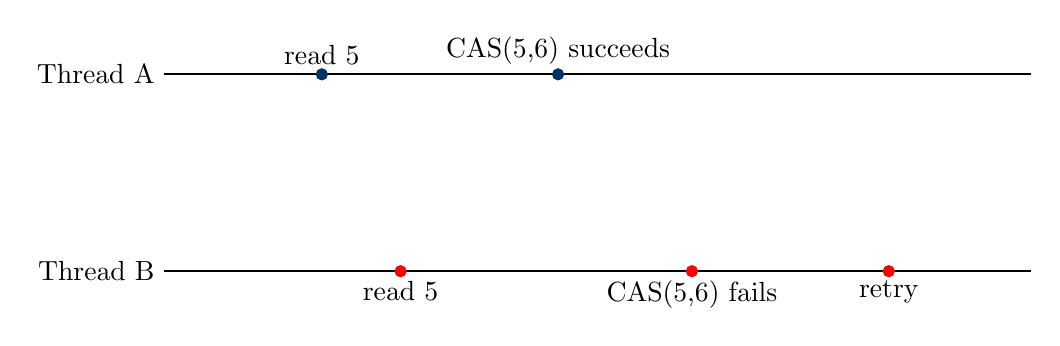
\begin{tikzpicture}[x=1cm,y=1cm]
			\draw[thick] (0,4) -- (11,4);
			\node[left] at (0,4) {Thread A};
			
			\draw[thick] (0,1.5) -- (11,1.5);
			\node[left] at (0,1.5) {Thread B};
			
			\filldraw[deepblue] (2,4) circle (2pt);
			\node[above] at (2,4) {read 5};
			
			\filldraw[deepblue] (5,4) circle (2pt);
			\node[above] at (5,4) {CAS(5,6) succeeds};
			
			\filldraw[red] (3,1.5) circle (2pt);
			\node[below] at (3,1.5) {read 5};
			
			\filldraw[red] (6.7,1.5) circle (2pt);
			\node[below] at (6.7,1.5) {CAS(5,6) fails};
			
			\filldraw[red] (9.2,1.5) circle (2pt);
			\node[below] at (9.2,1.5) {retry};
			
		\end{tikzpicture}
		
		\vspace{0.35cm}
		
		\begin{block}{Outcome}
			Only one update wins per expected state.  
			The loser retries with the new observed value.
		\end{block}
	\end{frame}
	
	% =========================================================
	\begin{frame}{What ``Lock-Free'' Means Here}
		\begin{block}{Introductory definition}
			A lock-free algorithm avoids traditional blocking locks and instead relies on atomic primitives such as CAS.
		\end{block}
		
		\vspace{0.35cm}
		
		\begin{exampleblock}{Practical classroom meaning}
			Threads do not wait to acquire a monitor or explicit lock for the update.  
			They attempt the update optimistically and retry if needed.
		\end{exampleblock}
		
		\vspace{0.3cm}
		
		\begin{alertblock}{Be careful}
			Lock-free does \emph{not} mean:
			\begin{itemize}
				\item no contention
				\item no retries
				\item always faster
				\item automatically simpler
			\end{itemize}
		\end{alertblock}
	\end{frame}
	
	% =========================================================
	\begin{frame}{Why Lock-Free Sounds Attractive}
		Lock-free approaches can offer benefits such as:
		
		\begin{itemize}
			\item no traditional lock acquisition on simple operations
			\item avoidance of some blocking overheads
			\item good scalability for some workloads
			\item reduced risk of classic lock-based waiting chains
		\end{itemize}
		
		\vspace{0.35cm}
		
		\begin{exampleblock}{Typical good use}
			Shared counters, simple flags with atomic transitions, and lightweight concurrent state updates.
		\end{exampleblock}
	\end{frame}
	
	% =========================================================
	\begin{frame}{But Lock-Free Also Has Costs}
		Lock-free is not magic.
		
		\vspace{0.3cm}
		
		Possible costs:
		\begin{itemize}
			\item repeated retries under contention
			\item wasted work when CAS fails repeatedly
			\item cache line bouncing across cores
			\item more subtle reasoning than plain sequential code
		\end{itemize}
		
		\vspace{0.35cm}
		
		\begin{alertblock}{Engineering reality}
			Under high contention, many threads may repeatedly fight over the same memory location.
		\end{alertblock}
	\end{frame}
	
	% =========================================================
	\begin{frame}{Contention: The Real Performance Question}
		\begin{block}{Contention}
			Contention occurs when many threads repeatedly access and update the same shared resource.
		\end{block}
		
		\vspace{0.35cm}
		
		For a shared counter, this means:
		\begin{itemize}
			\item multiple threads compete for one value
			\item multiple CAS attempts fail
			\item synchronization traffic increases
		\end{itemize}
		
		\vspace{0.35cm}
		
		\begin{exampleblock}{Key lesson}
			Concurrency performance is not about ideology.  
			It is about workload, contention level, and access pattern.
		\end{exampleblock}
	\end{frame}
	
	% =========================================================
	\begin{frame}{Low Contention vs High Contention}
		\begin{columns}[T]
			\column{0.48\textwidth}
			\begin{block}{Low contention}
				\begin{itemize}
					\item few collisions
					\item CAS often succeeds quickly
					\item atomics may perform very well
				\end{itemize}
			\end{block}
			
			\column{0.48\textwidth}
			\begin{block}{High contention}
				\begin{itemize}
					\item many collisions
					\item repeated CAS failures
					\item retries waste CPU work
				\end{itemize}
			\end{block}
		\end{columns}
		
		\vspace{0.35cm}
		
		\begin{alertblock}{Important}
			The same mechanism can look excellent in one scenario and poor in another.
		\end{alertblock}
	\end{frame}
	
	% =========================================================
	\begin{frame}{Comparison with Traditional Locks}
		\centering
		\begin{tabular}{>{\bfseries}m{3cm} m{6.8cm}}
			\texttt{synchronized} / \texttt{ReentrantLock} & serialize access to a critical section \\
			\texttt{AtomicInteger} & provides atomic operations on a value without a traditional lock block \\
			Lock-based update & wait / enter / execute / release \\
			CAS-based update & try / fail-or-succeed / retry if needed \\
		\end{tabular}
		
		\vspace{0.4cm}
		
		\begin{exampleblock}{Interpretation}
			Locks and atomics solve overlapping but not identical problems.
		\end{exampleblock}
	\end{frame}
	
	% =========================================================
	\begin{frame}{When Locks Are Still Better}
		Even after learning atomics, students should not think:
		\[
		\texttt{CAS solves everything}
		\]
		
		\vspace{0.35cm}
		
		Locks are still often better when:
		\begin{itemize}
			\item several variables must be updated together
			\item a larger critical section must remain consistent
			\item code clarity matters more than micro-optimization
			\item the logic is complex and retry-based reasoning becomes messy
		\end{itemize}
		
		\vspace{0.35cm}
		
		\begin{alertblock}{Important}
			Atomic classes are excellent for specific patterns, not for every concurrency design.
		\end{alertblock}
	\end{frame}
	
	% =========================================================
	\begin{frame}{When AtomicInteger Is a Great Fit}
		\texttt{AtomicInteger} is especially good for:
		
		\begin{itemize}
			\item counters
			\item sequence numbers
			\item simple state transitions
			\item lightweight shared metrics
		\end{itemize}
		
		\vspace{0.35cm}
		
		\begin{exampleblock}{Typical idea}
			One shared variable, one atomic operation, many concurrent updates.
		\end{exampleblock}
	\end{frame}
	
	% =========================================================
	\begin{frame}{Optional Extension: LongAdder}
		For strong students, you may mention:
		
		\[
		\texttt{LongAdder}
		\]
		
		\vspace{0.35cm}
		
		\begin{block}{Why it exists}
			Under very high contention, repeatedly updating one single atomic value can become a bottleneck.
		\end{block}
		
		\vspace{0.3cm}
		
		\begin{exampleblock}{General idea}
			Instead of forcing all threads to hit one shared point, work can be spread across multiple internal cells and combined later.
		\end{exampleblock}
		
		\vspace{0.25cm}
		
		This is an optimization topic, not the main core of Part 4.
	\end{frame}
	
	% =========================================================
	\begin{frame}{A Benchmark Mindset}
		Students should compare at least four counter strategies:
		
		\begin{enumerate}
			\item plain \texttt{int}
			\item \texttt{volatile int}
			\item synchronized counter
			\item \texttt{AtomicInteger}
		\end{enumerate}
		
		\vspace{0.35cm}
		
		For each version, measure:
		\begin{itemize}
			\item correctness of final result
			\item time under 2 threads
			\item time under 4, 8, or more threads
		\end{itemize}
		
		\vspace{0.35cm}
		
		\begin{alertblock}{Pedagogical benefit}
			Students stop arguing abstractly and start observing real tradeoffs.
		\end{alertblock}
	\end{frame}
	
	% =========================================================
	\begin{frame}{Counter Strategy Comparison}
		\centering
		\begin{tabular}{>{\bfseries}m{3.2cm} >{\centering\arraybackslash}m{1.8cm} >{\centering\arraybackslash}m{1.8cm} >{\centering\arraybackslash}m{2.1cm}}
			\toprule
			Strategy & Correct? & Blocks? & Good for \\
			\midrule
			Plain \texttt{int} & No & No & nothing concurrent \\
			\texttt{volatile int} & No for increment & No & visibility-only communication \\
			synchronized counter & Yes & Yes & critical sections \\
			\texttt{AtomicInteger} & Yes & No traditional lock & atomic value updates \\
			\bottomrule
		\end{tabular}
	\end{frame}
	
	% =========================================================
	\begin{frame}{What Students Must Not Conclude}
		They must \textbf{not} leave this lecture believing:
		
		\begin{itemize}
			\item ``lock-free always means faster''
			\item ``CAS never fails''
			\item ``AtomicInteger replaces locks in every design''
			\item ``retry is free''
		\end{itemize}
		
		\vspace{0.35cm}
		
		\begin{alertblock}{Replace with}
			\begin{quote}
				Atomics are powerful for specific update patterns, but performance and suitability depend on contention and design structure.
			\end{quote}
		\end{alertblock}
	\end{frame}
	
	% =========================================================
	\begin{frame}{Part 4 Concept Summary}
		\centering
		\begin{tabular}{>{\bfseries}m{3cm} m{7.1cm}}
			\texttt{AtomicInteger} & atomic shared-value operations in Java \\
			CAS & compare current value and swap only if expectation still matches \\
			Optimistic update & try update first, retry if interference occurred \\
			Lock-free idea & avoid traditional blocking locks for some operations \\
			Contention & many threads competing for the same shared state \\
			Engineering lesson & no tool is universally best \\
		\end{tabular}
	\end{frame}
	
	% =========================================================
	\begin{frame}{Lab Preparation for Part 4}
		\begin{block}{Lab 4.8 --- Atomic Counter}
			Students replace an unsafe counter with \texttt{AtomicInteger} and verify correctness.
		\end{block}
		
		\vspace{0.25cm}
		
		\begin{block}{Lab 4.9 --- CAS Retry Demo}
			Students manually code a retry loop using:
			\begin{itemize}
				\item \texttt{get()}
				\item \texttt{compareAndSet()}
			\end{itemize}
		\end{block}
		
		\vspace{0.25cm}
		
		\begin{block}{Lab 4.10 --- Contention Benchmark}
			Students compare:
			\begin{itemize}
				\item plain int
				\item volatile int
				\item synchronized counter
				\item AtomicInteger
			\end{itemize}
			under several thread counts.
		\end{block}
	\end{frame}
	
	% =========================================================
	\begin{frame}{Suggested Discussion Questions}
		\begin{enumerate}
			\item Why is \texttt{AtomicInteger} different from \texttt{volatile int}?
			\item What does CAS actually check?
			\item Why must a failed CAS retry?
			\item What does lock-free mean in practical terms?
			\item Why might atomics perform poorly under high contention?
			\item When would a lock still be the clearer or safer solution?
		\end{enumerate}
	\end{frame}
	
	% =========================================================
	\begin{frame}{Week 4 Final Synthesis}
		\centering
		\begin{tabular}{>{\bfseries}m{2.8cm} m{7.4cm}}
			Part 1 & why threads can observe stale memory \\
			Part 2 & how \texttt{volatile} provides visibility and ordering \\
			Part 3 & why visibility is not enough; atomicity and DCL \\
			Part 4 & how atomics and CAS support lock-free updates \\
		\end{tabular}
		
		\vspace{0.45cm}
		
		\begin{exampleblock}{The real progression}
			\begin{enumerate}
				\item Threads can disagree about memory
				\item Visibility can be restored
				\item Visibility is not atomicity
				\item Atomic updates can be built with CAS
			\end{enumerate}
		\end{exampleblock}
	\end{frame}
	
	% =========================================================
	\begin{frame}{Final Takeaway of the Whole Week}
		\begin{alertblock}{Week 4 takeaway}
			Concurrent correctness depends on three different questions:
			\begin{itemize}
				\item What can threads see?
				\item In what order can they see it?
				\item Does an update happen as one indivisible action?
			\end{itemize}
		\end{alertblock}
		
		\vspace{0.35cm}
		
		\begin{block}{Tool map}
			\begin{itemize}
				\item \texttt{volatile} helps with visibility and ordering
				\item locks help with mutual exclusion and grouped atomicity
				\item atomic classes help with lock-free atomic updates
			\end{itemize}
		\end{block}
	\end{frame}
	
	% =========================================================
	\begin{frame}{End of Part 4}
		\centering
		\Huge Questions?
	\end{frame}
	
	% =========================================================
\end{document}